\documentclass[crop,tikz]{standalone}
	\usetikzlibrary{patterns}
\begin{document}
	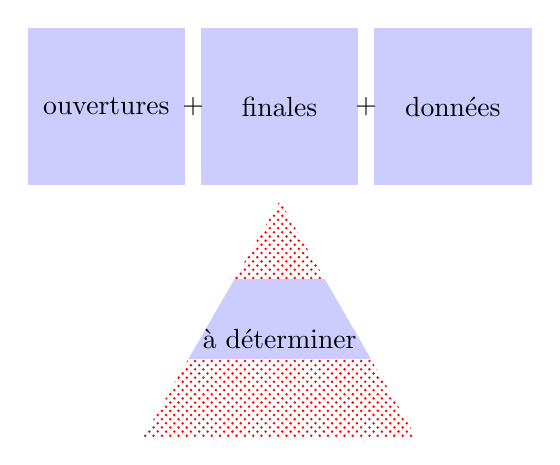
\begin{tikzpicture}
		\fill[color=blue!20] (-3.2, 2.2) rectangle (-1.2,4.2) node[color=black,pos=.5] {ouvertures};
		\fill[color=blue!20] (-1, 2.2) rectangle (1,4.2) node[color=black,pos=.5] {finales};
		\fill[color=blue!20] (1.2, 2.2) rectangle (3.2,4.2) node[color=black,pos=.5] {donn\'{e}es};
		\draw (-1.1,3.2) node{$+$} ;
		\draw (1.1,3.2) node{$+$} ;
		
 		\begin{scope}
 		\clip (-1,1) rectangle (1,2);
 		\fill[pattern=crosshatch dots, pattern color=red] (90:2cm) \foreach \x in {210,330} {
 			-- (\x:2cm)
 		} -- cycle (0,0) ;
 		\end{scope}
 		
		\begin{scope}
			\clip (-2,0) rectangle (2,1);
			\fill[color=blue!20] (90:2cm) 
			\foreach \x in {210,330} {
				-- (\x:2cm)
			} -- cycle (0,0) node[color=black,above]{\`{a} d\'{e}terminer} ;
		\end{scope}
		
		\begin{scope}
			\clip (-2,-1) rectangle (2,0);
			\fill[pattern=crosshatch dots, pattern color=red] (90:2cm) \foreach \x in {210,330} {
				-- (\x:2cm)
			} -- cycle (0,0) ;
		\end{scope}
	\end{tikzpicture}
\end{document}